\documentclass[a4paper,12pt]{article}
\usepackage[latin1]{inputenc}
\usepackage{graphicx}
\usepackage[T1]{fontenc}
\usepackage[spanish]{babel}
\usepackage{hyperref}

\title{%

An\'alisis de tendencias sociales.%
	
	\author{%
	Enrique Vilanova Vidal%
		\thanks{Todos los que han colaborado en el proyecto}
	\and Brais Suarez Souto
		\thanks{Las comunidades online que nos han permitido realizar este trabajo}
	}

}



\begin{document}


\maketitle
\thispagestyle{empty}
\clearpage
\pagenumbering{arabic} 
\newpage



\section[item_contexto]{Contexto}

En una sociedad en constante y  r\'apido cambio es importante entender las {\itshape tendencias sociales} de un momento en particular y poder pronosticar su posible evoluci\'on.
Entendiendo por  {\itshape tendencia social} algo que es importante para un segmento de la poblaci\'on o mercado en un momento dado.

?`Qu\'e hace a algo relevante para  la sociedad?  esta pregunta cl\'asica  est\'a en el coraz\'on de muchas disciplinas sociales. Disciplinas que van desde la {\itshape sociolog\'ia} puramente acad\'emica hasta disciplinas aplicadas c\'omo {\itshape marketing publicitario}, para todas ellas es fundamental encontrar alg\'un tipo de respuesta a la pregunta acerca de lo que interesa a la sociedad.

Esta pregunta ha sido abordada hasta la fecha, desde un punto de vista matem\'atico, por modelos {\itshape theory-driven}~\cite{td1,td2,td3}. Los recientes avances en inteligencia artificial y la abundancia de informaci\'on disponible en Internet, hace posible intentar responder a la misma pregunta cl\'asica, pero esta vez con modelos {\itshape data-driven}\cite{dd1}.

Contestar de forma general, ?`Qu\'e hace a algo relevante para  la sociedad? es un primer paso muy ambicioso por lo que es razonable elegir un contexto acotado, por lo que, en concreto nos preguntamos por:

\begin{itemize}

\item Espa\~na
\item Noticias
\item Actualidad

\end{itemize}

En este sentido, consideramos relevante obtener informaci\'on de agregadores de noticias y foros o redes sociales, donde sea razonable pensar que son los usuarios los que eligen qu\'e tema es relevante.

Meneame es el mayor agregador de noticias de Espa\~na. Obteniendo datos de su secci\'on {\itshape portada} podemos tener informaci\'on de las noticias de actualidad que han sido relevantes. Adem\'as, Meneame ofrece una secci\'on {\itshape nuevas} donde podemos ver  la mayor\'ia de las noticias subidas por los usuarios. Comparando {\itshape portada} y {\itshape nuevas} podemos intentar entender las diferencias entre las noticias que llegaron a portada y las que no. {\itshape A priori}, entendemos que las noticias que llegan a {\itshape portada}  han sido m\'as relevantes para la mayor\'ia de los usuarios.

Utilizaremos otras webs que funcionan como agregadores de noticias, con el fin de minimizar el sesgo proveniente del hecho de que los usuarios de Meneame pueden estar concentrados en un segmento espec\'ifico de la poblaci\'on. Adem\'as tambi\'en se estudiar\'a el impacto de la noticia en redes sociales.

Para el prop\'osito de esta pr\'actica presentamos los datos provenientes de:

\begin{itemize}
\item Meneame: {\itshape portada}.
\item Reddit: {\itshape subreddits de noticias de actualidad sobre Espa\~na}.
\item Twitter: las {\itshape tags} extra\'idas de las noticias se usan para estudiar el impacto de la noticia. 

\end{itemize}

La informaci\'on de Meneame se ha extra\'ido con {\itshape web scrapping} (pese a contar con API) como ejercicio acad\'emico (practicar). Adem\'as, puede ser interesante usar  {\itshape web scrapping} como forma de evitar las limitaciones impuestas por las API.

\section[item_titulo]{T\'itulos}


\begin{itemize}

\item Noticias {\itshape portada} Meneame.
\item Noticias Reddit Espa\~na.
\item Tweets por {\itshape tag}.


\end{itemize}

\section[item_dataset]{Datasets}

Se trata de tres datasets, provenientes de tres fuentes diferentes, Meneame, Twitter, y Reddit. Para los tres datasets se ha capturado el m\'aximo de informaci\'on relevante con el fin de realizar un estudio de la relevancia de la noticia. Entre otras cosas se pretende estudiar:

\begin{itemize}

\item El tiempo que tarde una noticia en convertirse en relevante.
\item Los factores comunes en noticias relevantes.
\item N\'umero de usuarios relacionados con la noticia (comentan, twittean...)
\item Sentimiento en la noticia y hacia la noticia.
\item Reconocimiento {\itshape nombre-entidad} en la noticia.
\item Estratificaci\'on de usuarios de acuerdo a una noticia
\item Estudio comparativo usuarios con distribuciones poblaci\'on extra\'idos de otras fuentes (INE).  
\end{itemize}


\section[item_grafico]{Representaci\'on  gr\'afica. }

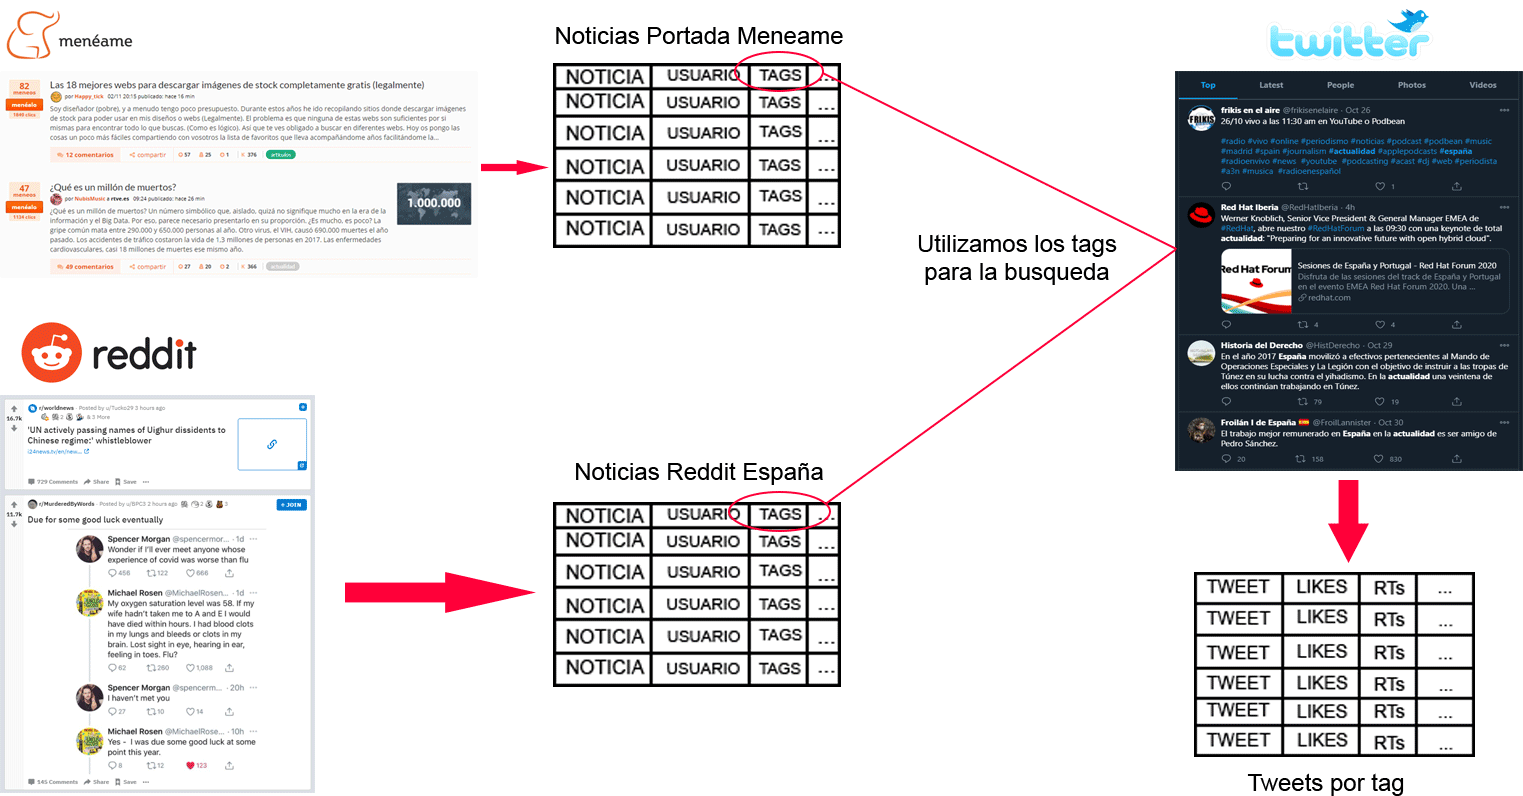
\includegraphics[scale = 0.25]{esquema.png}

\section[item_contenido]{Contenido}

\subsection{Meneame}

El dataset para Meneame se ha hecho utilizando {\itshape Python} y la librer\'ia {\itshape Beautifulsoup}. Meneame dispone de una API, pero por motivos acad\'emicos y con la intenci\'on de presentar un trabajo lo m\'as completo posible, para el caso de Meneame no se ha utilizado la API.

Cabe remarcar, que tal como se puede ver en el c\'odigo del scrapper, para cada noticia se genera un segundo dataset con los comentarios de cada usuario para una noticia en concreto, as\'i como otra informaci\'on relevante de la noticia. Se elige esta aproximaci\'on para mantener el dataset principal legible, siendo el dataset principal el obtenido de Meneame {\itshape portada}. Toda la informaci\'on puede accederse a trav\'es de una base de datos relacional. Aunque los datasets espec\'ifcos de cada noticia no se incluyen en el trabajo.

 
\begin{itemize}

\item C\'odigo: clave principal de la noticia.
\item Titular: titular de la noticia.
\item Fecha de env\'io: hora a la que noticia es enviada a Meneame.
\item Publicada: hora a la que la noticia es publicada
\item Web origen: origen de la noticia
\item C\'odigo usuario: clave num\'erica for\'anea que permite identificar a usuarios
\item Nick: nombre del usuario
\item Tema principal: primera etiqueta descriptiva de la noticia
\item Columnas Sub Tema: todas las otras posibles clasificaciones que el usuario aporta para una noticia
\item  Clicks: n\'umero de veces que se ha clicado en la noticia
\item Positivos": n\'umero de votos positivos ofrecidos por usuarios registrados
\item An\'onimos: n\'umero de votos positivos ofrecidos por usuarios no registrados
\item Negativos: n\'umero de votos negativos
\item Karma: factor de relevancia num\'erico asignado por Meneame
\item N\'umero de comentarios: n\'umero de comentarios que tiene una noticia

\end{itemize}


\subsection{Reddit}

El objetivo de este dataset es hacer una comprobaci\'on cruzada con las noticias extra\'idas de Meneme y ver si tambi\'en han sido relevantes en Reddit y que grado de relevancia han tenido.Tambi\'en se quiere buscar posibles noticias relevantes que no hayan llegado a {\itshape portada} de Meneame pero si hayan sido relevantes. Adem\'as de comparar el sentimiento de los comentarios hacia las noticias (entre otras cosas).

Desafortunadamente, Reddit tiene una repercusi\'on (en n\'umero de usuarios activos) menor que Meneame. Para evaluar los datos, esto a\~nade la dificultad de definir un factor de peso para las noticias dependiendo del medio.

En el c\'odigo del scrapper tambi\'en se ha tenido en cuenta que Reddit no tiene secci\'on {\itshape portada} y {\itshape nuevas} (como Meneame) por lo que se ha incluido una primer filtro donde \'unicamnete se seleccionan noticias que han tenido una cierta cantidad de votos positivos (ser\'ia nuestro equivalente a {\itshape portada}). Esto se ha hecho por motivos de consistencia con el dataset que se entrega de Meneame, ya que este solo incluye las noticias de {\itshape portada}. Otra cosa a tener en cuenta es que las noticias de Reddit no tienen {\itshape tags} proporcionadas por los usuarios, sin embargo los subreddits escogidos, podr\'ian ser todos categorizados por las {\itshape tags}; noticias, actualidad, Espa\~na.

Al igual que en el caso anterior, en el c\'odigo del scrapper se puede ver como se genera un segundo dataset con todos los comentarios de cada noticia y otra informaci\'on relevante, que no se presenta pero se incluye en nuestra base de datos relacional.  

Para este caso y por sencillez hemos escogido realizar el scrapping usando la API de Reddit.


Descripci\'on de los atributos:

\begin{itemize}

\item Id del post: clave principal para identificar el post.

\item T\'itulo: t\'itulo del post.

\item ups: votos  positivos o ups.

\item downs: vostos negativos o downs.

\item N\'umero de comentarios: cantidad de comentarios para una noticia.

\item Autor: autor del post.

\item Fecha: fecha en la que se cre\'o el post.

\item link: enlace a la web de origen de la noticia.

\item subreddit: subreddit donde se ha extra\'ido el post.
\end{itemize}


\subsection{Twitter}

El scrapper de Twitter se utiliza para seguir la relevancia de las noticias en un medio generalista. Se usan las{\itshape tags} extra\'idas de las noticias para comprobar su relevancia. En primer paso, las tags se seleccionan manualmente y se compruebar\'a de forma manual que los twits correspondan a cierto tema. El prop\'osito final es automatizar todo el proceso, lo que presenta el desaf\'io de comprobar que ciertos tweets corresponden a un tema en concreto. Sin entrar en detalles, para afrontar este desaf\'io se usar\'a redes neuronales para la identificaci\'on de {\itshape nombre-entidad} en el cuerpo de las noticias, con el fin de generar vectores de proximidad, as\'i como {\itshape contextual topic recognition}.

Para el prop\'osito de esta pr\'actica se entrega el dataset correspondiente a dos noticias, donde las {\itshape tags} se han seleccionado (manualmente), a partir de las {\itshape tags} que los usuarios de Meneame proporcionan para describir una noticia.

Descripci\'on del dataset:

\begin{itemize}

\item query: La query usada para generar el dataset.

\item Tweet ID: ID del Tweet.

\item Text: Texto del Tweet.

\item RT Count: N\'umero de veces que el Tweet ha sido retweeteado.

\item Username: Nombre de usuario del autor del Tweet.

\item Likes: N\'umero de veces que el Tweet ha recibido un like.

\item Created at: fecha en la que se cre\'o el Tweet.

\end{itemize}

\subsection{Otros}

A medida que avance el proyecto otros foros y plataformas se ir\'an incluyendo, cabe mencionar especialmente {\itshape Facebook} por su cantidad de usuarios.

Es importante mencionar, que con el fin de estimar apropiadamente, las distribuciones de poblaci\'on (entre otros), se consultar\'an bases de datos del {\itshape INE}. 

\section{Agradecimientos}

Agradecimientos a las plataformas de Meneame, Reddit y Twitter por permitirnos utilizar sus plataformas y recursos para obtenci\'on de datos generados en ellas.

Nos gustar\'ia agradecer especialmente a los miembros de su comunidad por su participaci\'on en las distintas plataformas ya que hacen posible este tipo de trabajos que una d\'ecada atr\'as hubiese requerido de una gran cantidad de capital para entrevistar a una parte significativa de la poblaci\'on.

\subsection{Reddit y Twitter}

El scrapping de estos sitios webs se ha realizado a trav\'es de sus API para python. En ambos casos se ha utilizado una cuenta de desarrollador y nos hemos mantenido dentro de las limitaciones especificadas (n\'umero de peticiones por minuto y n\'umero de twits por hora)

\subsection{Meneame}

Para el caso Meneame nos hemos mantenido dentro de los l\'imites especificados en el archivo robots.txt. En este archivo, se permite todos los {\itshape user agent}. No ha sido necesario acceder a ninguna de las carpetas que figuran como {\itshape Disallow}.


\section{Inspiraci\'on}

C\'omo ya se ha mencionado la pregunta que se intenta responder es ?`Qu\'e hace a algo relevante para la sociedad?, pero tambi\'en se quiere averiguar ?`Qu\'e temas son relevantes para la sociedad, en este momento?, ?`Por cuanto tiempo se mantiene  relevante? Este tipo de preguntas son fundamentales en muchas \'areas, tanto acad\'emicas como relacionadas con los negocios. Poder contestar satisfactoriamente estas preguntas, podr\'ia permitir, entre otras cosas, planificar adecuadamente campa\~nas publicitarias dirigidas a un segmento de la poblaci\'on y sabiendo cuanto tiempo han de extenderse en el tiempo. As\'i c\'omo reaccionar en tiempo real al cambio de opiniones y gustos.

\section{Licencia}

Todo el material entregado en esta pr\'actica est\'a bajo licencia:

\begin{itemize}

\item Released Under CC0: Public Domain License


\end{itemize}

Debido a que nosotros estamos form\'andonos, y estamos utilizando contenido generado por comunidades de usuarios abiertas y todav\'ia no contiene ning\'un an\'alisis, vamos a lanzar nuestro dataset con licencia CC0, por lo tanto rechazamos cualquier tipo de derechos sobre la autor\'ia del mismo, para que cualquier persona interesada pueda trabajar con \'el y hacerlo suyo, sin necesidad de darnos ning\'un tipo de atribuci\'on.  M\'as informaci\'on se puede encontrar en la p\'agina oficial de CC.
https://creativecommons.org/share-your-work/public-domain/cc0/

\section{C\'odigo}

Todo el c\'odigo utilizado para el desarrollo de los scrappers puede encontrarse en la carpeta Scrapper del repositorio de \href{https://github.com/Envivi-git/News_analysis.git}{gitHub}.

\section{Dataset}

Enlaces: 

\begin{itemize}

\item Siguiendo el \href{https://zenodo.org/record/4243130}{Link} se  pueden encontrar los datasets de Reddit y Meneame con DOI 10.5281/zenodo.4243130 subidos a Zenodo. El dataset de Twitter no se ha subido a Zenodo ya que tiene un c\'aracter de an\'alisis mas espec\'ifico, pero se ha incluido dentro del repositorio de github.

\item Usando este \href{https://github.com/Envivi-git/News_analysis/tree/main/Dataframes_CSV}{link}  se puede encontrar el repositorio de GitHub d\'onde se han subido los \'ultimos datasets generados. 

\end{itemize}

\section{Participaci\'on}

\begin{tabular}{|l|c|c|}\hline

Actividad& Integrante 1& Integrante 2\\\hline
Investigaci\'on previa & Enrique Vilanova & Brais Su\'arez \\\hline
Redacci\'on de las respuestas & Enrique Vilanova & Brais Su\'arez \\\hline
Desarrollo c\'odigo  & Enrique Vilanova & Brais Su\'arez \\\hline

\end{tabular}

\begin{thebibliography}{9}

\bibitem{td1} Leonard Berzkowitz,%
	\emph{ Advances in Experimental Social Psychology}, 1967,  Academic press
\bibitem{td2} Richard McElreath, Robert Boyd,%
	\emph{ Mathematical Models of Social Evolution: A Guide for the Perplexed}, 2007, The University of Chicago Press
\bibitem{td3}Thomas L. Saaty and Joyce M. Alexander,%
	\emph{Thinking with models: Mathematical Models in the Physical, Biological, and Social Sciences}, 2015, RWS Publications
\bibitem{dd1}Jason Radford and Kenneth Joseph,%
	\emph{Theory In, Theory Out: The Uses of Social Theory in Machine Learning for Social Science}, 2020, doi.org/10.3389/fdata.2020.00018

\end{thebibliography}

\end{document}



